\documentclass[11pt,a4paper]{article}

\usepackage[utf8]{inputenc}
\usepackage[margin=0.62in,top=0.60in,bottom=0.62in]{geometry}
\usepackage{amsmath,amssymb}
\usepackage{tabularx}
\usepackage{array}
\usepackage{graphicx}
\usepackage{color}
\usepackage{url}
\usepackage{fancyhdr}
\usepackage{keyval}
\usepackage{hyperref}

\graphicspath{{results/figures/}{figures/}{./}}

% Harmonious color palette
\definecolor{primaryblue}{rgb}{0.09, 0.30, 0.47}
\definecolor{accentgreen}{rgb}{0.13, 0.55, 0.13}
\definecolor{accentred}{rgb}{0.70, 0.13, 0.13}
\definecolor{lightgray}{gray}{0.96}
\definecolor{boxgray}{gray}{0.94}
\definecolor{darkgray}{gray}{0.25}

% Clean table rule fallbacks
\providecommand{\toprule}{\hline\hline}
\providecommand{\midrule}{\hline}
\providecommand{\bottomrule}{\hline\hline}

% Clickable hyperlinks
\hypersetup{
  colorlinks=true,
  linkcolor=primaryblue,
  urlcolor=primaryblue,
  citecolor=primaryblue,
  pdfborder={0 0 0}
}

% Tight spacing
\setlength{\headheight}{14pt}
\addtolength{\topmargin}{-2pt}
\setlength{\parskip}{1.6pt plus 0.4pt minus 0.3pt}
\setlength{\parindent}{0pt}
\raggedbottom

% Custom non-floating captions
\makeatletter
\newcommand{\captionof}[2]{%
  \def\@captype{#1}%
  \caption{#2}%
}
\renewcommand\section{\@startsection{section}{1}{\z@}%
  {-1.0ex \@plus -0.2ex \@minus -.1ex}%
  {0.4ex \@plus .1ex}%
  {\normalfont\large\bfseries\color{primaryblue}}}
\renewcommand\subsection{\@startsection{subsection}{2}{\z@}%
  {-0.8ex\@plus -0.2ex \@minus -.1ex}%
  {0.25ex \@plus .1ex}%
  {\normalfont\normalsize\bfseries\color{primaryblue}}}
\makeatother

% Tight center environment to remove excessive vertical margins around tables & plots
\newenvironment{tightcenter}{%
  \setlength\topsep{1.2pt}%
  \setlength\parskip{0pt}%
  \begin{center}%
}{%
  \end{center}%
}

% Case study box macro
\newcommand{\casebox}[4]{%
  \vspace{0.08em}%
  \noindent\fcolorbox{primaryblue}{boxgray}{%
    \begin{minipage}{\dimexpr\linewidth-2\fboxsep-2\fboxrule\relax}%
      \textbf{\color{primaryblue}#1} \hfill \textbf{\footnotesize #4}\par\vspace{0.04em}\hrule\vspace{0.08em}%
      \textbf{Query:} \textit{``#2''}\\[0.06em]%
      \textbf{Expected Answer:} #3%
    \end{minipage}%
  }%
  \vspace{0.08em}%
}

% Header and Footer
\pagestyle{fancy}
\fancyhf{}
\lhead{\textbf{LMA Assignment 1}}
\rhead{\textbf{2023101102}}
\cfoot{\thepage}

\begin{document}

% =================================================================================================
% PAGE 1: TITLE, INTRODUCTION, ARCHITECTURE COMPARISON, INGESTION
% =================================================================================================
\begin{tightcenter}
  {\LARGE\textbf{LMA Assignment 1}}\\[0.15em]
  {\large Raghav Grover, 2023101102 \quad|\quad \textbf{GitHub:} \url{https://github.com/RaghavgitGrover/LMA_A1}}
\end{tightcenter}
\vspace{-0.4em}
\hrule
\vspace{0.35em}

\section{Introduction}
\label{sec:intro}
This report implements, evaluates, and benchmarks a two-stage RAG pipeline over the official text of \textit{The Constitution of India} (pages 32--381, 880 semantic chunks). We evaluate two distinct retrieval workflows against a curated ground-truth benchmark of 56 legal queries:
\begin{enumerate}
  \setlength{\itemsep}{0.5pt}\setlength{\parskip}{0pt}
  \item \textbf{Pipeline 1 (Baseline Vector Retrieval):} Encodes passages and incoming queries independently into 384-dimensional dense vectors using a Bi-Encoder (BE, \texttt{all-MiniLM-L6-v2}), retrieves Top-10 candidates via inner product search in a flat FAISS index, and feeds Top-3 candidates directly to a local LLM (\texttt{llama3.2:3b} via Ollama, temperature $= 0$) to produce \textbf{Answer 1}.
  \item \textbf{Pipeline 2 (CE Re-Ranking):} Passes Top-10 candidates from Stage 1 into a local Cross-Encoder (CE, \texttt{ms-marco-MiniLM-L6-v2}) for joint token-level cross-attention scoring, re-ranks candidates descending by relevance logit, and supplies Top-3 re-ordered candidates to the same LLM to produce \textbf{Answer 2}.
\end{enumerate}
We analyze retrieval accuracy improvements, qualitative failure modes, stage-wise latency profiles, and the theoretical computational limits of exhaustive cross-encoding.

\section{Architecture Comparison: BE vs.\ CE}
\label{sec:architecture}

\subsection{BE: Fast First-Stage Vector Retrieval}
\begin{itemize}
  \setlength{\itemsep}{0pt}\setlength{\parskip}{0pt}\setlength{\parsep}{0pt}
  \item \textbf{Model \& Index:} \texttt{all-MiniLM-L6-v2} ($d = 384$, 22.7M parameters) paired with FAISS \texttt{IndexFlatIP} (exact inner product on unit-normalized vectors).
  \item \textbf{Mechanism \& Role:} Chunks are pre-embedded offline and indexed. At inference, query encoding ($9.88$\,ms) plus FAISS vector search ($0.14$\,ms) evaluates $s(q, d) = \mathbf{u}_q^\top \mathbf{v}_d$ over all 880 chunks to generate Top-10 candidates at sub-millisecond retrieval latency ($880 \rightarrow 10$).
\end{itemize}

\subsection{CE: Precise Second-Stage Re-Ranking}
\begin{itemize}
  \setlength{\itemsep}{0pt}\setlength{\parskip}{0pt}\setlength{\parsep}{0pt}
  \item \textbf{Model \& Scoring:} \texttt{ms-marco-MiniLM-L6-v2} (22.7M parameters) jointly processes concatenated sequence \texttt{[CLS]} $\circ\, q \,\circ$ \texttt{[SEP]} $\circ\, d \,\circ$ \texttt{[SEP]} through full token-level cross-attention across all 6 transformer layers.
  \item \textbf{Mechanism \& Role:} Directly outputs unconstrained scalar relevance logits for the 10 query-candidate pairs ($324.97$\,ms), sorting descending and supplying Top-3 chunks ($10 \rightarrow 3$) to the LLM prompt to resolve fine-grained statutory provisos.
\end{itemize}

\begin{tightcenter}
\small
\renewcommand{\arraystretch}{0.84}
\begin{tabularx}{\textwidth}{l p{5.5cm} X}
\toprule
\textbf{Dimension} & \textbf{BE (Pipeline 1)} & \textbf{CE (Pipeline 2 Stage b)} \\
\midrule
\textbf{Model} & \texttt{all-MiniLM-L6-v2} & \texttt{ms-marco-MiniLM-L6-v2} \\
\textbf{Representation} & Independent 384-d dense vectors & Joint query-document token sequence \\
\textbf{Scoring} & Inner product (cosine similarity) & Joint cross-attention scalar logit \\
\textbf{Precomputation} & Chunks precomputed and indexed offline & Dynamic per-query scoring; no precomputation \\
\textbf{Query Latency} & $10.02$\,ms ($N = 880$ chunks) & $324.97$\,ms ($k = 10$ candidate pairs) \\
\textbf{Operational Role} & Broad first-stage recall ($N = 880 \rightarrow 10$) & Precise second-stage re-ranking ($k = 10 \rightarrow 3$) \\
\bottomrule
\end{tabularx}
\vspace{0.08em}
\captionof{table}{Operational comparison of BE and CE in the RAG pipeline.}
\label{tab:arch_comparison}
\end{tightcenter}

\subsection{Document Ingestion, Cleaning, and Validated Chunking}
The evaluation corpus is the official \textit{The Constitution of India}. We index pages 32 to 381 (1-indexed), omitting preliminary contents and end appendices:
\begin{enumerate}
  \setlength{\itemsep}{0pt}\setlength{\parskip}{0pt}\setlength{\parsep}{0pt}
  \item \textbf{Layout Preservation:} Extracted via \texttt{pdftotext -layout} to preserve clause indentation, paragraph breaks, and marginal numbering.
  \item \textbf{Footnote Sanitization:} Strips amendment footnotes strictly in bottom 55\% of each page ($i \ge 0.45 \cdot \text{total\_lines}$) to avoid truncating legal body text.
  \item \textbf{Unit Chunking:} Formatted into semantic chunks with target size \texttt{CHUNK\_CHARS} $= 900$ and overlap \texttt{CHUNK\_OVERLAP} $= 150$. Each chunk records \texttt{chunk\_id}, \texttt{article}, \texttt{articles}, and page bounds.
  \item \textbf{Sanity Verification:} Confirms $N = 880$ chunks, mean length $886$\,chars ($\min = 285$, $\max = 1050$), with 879/880 carrying verified Article metadata.
\end{enumerate}

\clearpage

% =================================================================================================
% PAGE 2: PIPELINE WORKFLOW, PROMPT FORMULATION, BENCHMARK DESIGN, HEADLINE METRICS
% =================================================================================================
\section{System Implementation and Experimental Design}
\label{sec:implementation}

\subsection{Two-Stage Pipeline Workflow}
Both RAG pipelines query the identical 880-chunk corpus under controlled generation settings:
\begin{itemize}
  \setlength{\itemsep}{0.5pt}\setlength{\parskip}{0pt}
  \item \textbf{Pipeline 1 (Baseline):} Retrieve Top-10 chunks via FAISS; feed Top-3 chunks directly to Llama-3.2-3B to produce \textbf{Answer 1}.
  \item \textbf{Pipeline 2 (Re-Ranked):} Re-score Top-10 candidates with CE; sort descending; feed Top-3 chunks to Llama-3.2-3B to produce \textbf{Answer 2}.
\end{itemize}

\subsection{Prompt Engineering and Context Injection}
Both pipelines use an identical prompt template to guarantee rigorous experimental control:

\vspace{0.06em}
\noindent\fcolorbox{primaryblue}{lightgray}{%
  \begin{minipage}{\dimexpr\linewidth-2\fboxsep-2\fboxrule\relax}
    \footnotesize
    \textbf{\color{primaryblue}System and Context Prompt Formulation}\par\vspace{0.04em}\hrule\vspace{0.08em}
    \textbf{System Prompt:}\\
    \textit{``You are a careful legal assistant for the Constitution of India. Answer the question using ONLY the context passages provided. If the context does not contain the answer, reply exactly: 'The provided context does not contain the answer.' Be concise (at most 4 sentences) and cite Article numbers when the context states them.''}\\[0.08em]
    \textbf{User Context Template:}\\
    \textsf{Context passages from the Constitution of India:}\\
    \textsf{[Passage 1 | chunk <id> | page <p>] <chunk text>}\quad
    \textsf{\dots}\quad
    \textsf{Question: <query> \quad $\longrightarrow$ \quad Answer:}
  \end{minipage}%
}
\vspace{0.06em}

\subsection{Benchmark Design: 56 Curated Ground-Truth Queries}
We constructed a balanced benchmark of \textbf{56 curated queries} across eight categories (7 queries each), annotated with expected answers, exact Article citations, required atomic facts, and unanswerable status.

\begin{tightcenter}
\footnotesize
\renewcommand{\arraystretch}{0.90}
\begin{tabularx}{\textwidth}{l p{3.2cm} X}
\toprule
\textbf{Category} & \textbf{Intent} & \textbf{Representative Benchmark Query} \\
\midrule
\textbf{Control (C1--C7)} & Direct single-article recall & \textit{C3: How long can an arrested person be detained before magistrate production, and what journey-time exception applies?} \\
\textbf{Keyword Trap (K1--K7)} & Lexical divergence & \textit{K5: Can police force of one State investigate or exercise jurisdiction in another State without permission?} (7th Sched., List I, Entry 80) \\
\textbf{Exception (E1--E7)} & Overridden general rules & \textit{E5: Under what circumstances can Parliament legislate on a State List subject in national interest?} (Art. 249(1)) \\
\textbf{Negation (N1--N7)} & Negative constraints \& bars & \textit{N5: What are the specific constitutional grounds for disqualification from being an MP?} (Art. 102(1)) \\
\textbf{Role Limit (R1--R7)} & Age thresholds \& quotas & \textit{R2: What is the minimum age to become a member of the Council of States?} (Art. 84(b): 30 years) \\
\textbf{Procedure (P1--P7)} & Multi-step mechanisms & \textit{P1: What majority is required in Parliament to pass an amendment under Article 368?} (Art. 368(2): Total majority + 2/3 voting) \\
\textbf{Cross-Article (X1--X7)} & Comparative synthesis & \textit{X1: How does pardoning power of President compare with Governor regarding death sentences?} (Art. 72 vs. Art. 161) \\
\textbf{Unanswerable (U1--U7)} & Out-of-corpus queries & \textit{U1: What is the mandatory retirement age for the President of India?} (No constitutional age limit; tests abstention) \\
\bottomrule
\end{tabularx}
\vspace{0.10em}
\captionof{table}{The 56-query legal evaluation benchmark across eight balanced categories.}
\label{tab:query_categories}
\end{tightcenter}

\section{Quantitative Retrieval Evaluation}
\label{sec:quantitative}

\subsection{Headline Retrieval Metrics}
Table~\ref{tab:headline_metrics} summarizes retrieval performance on the 48 answerable queries ($95\%$ bootstrap CI, $B=1,000$).

\begin{tightcenter}
\footnotesize
\setlength{\tabcolsep}{4pt}
\renewcommand{\arraystretch}{0.93}
\begin{tabular}{lcccccc}
\toprule
\textbf{Pipeline} & \textbf{Recall@10} & \textbf{Hit@3} & \textbf{MRR@10} & \textbf{nDCG@3} & \textbf{Mean Rank} & \textbf{Net Shift} \\
\midrule
\textbf{Baseline} & $0.833$ & $0.604$ & $0.524$ & $0.457$ & $4.19$ & --- \\
\textit{95\% Bootstrap CI} & --- & $[0.458, 0.750]$ & $[0.409, 0.640]$ & $[0.343, 0.578]$ & --- & --- \\
\midrule
\textbf{Re-Ranked} & $\mathbf{0.833}$ & $\mathbf{0.750}$ & $\mathbf{0.636}$ & $\mathbf{0.604}$ & $\mathbf{3.42}$ & $\mathbf{+18.8\%}$ \\
\textit{95\% Bootstrap CI} & --- & $[0.625, 0.855]$ & $[0.524, 0.752]$ & $[0.489, 0.711]$ & --- & (9 rescued) \\
\midrule
\textbf{Delta / Net Impact} & $0.000$ & $\mathbf{+14.6\%}$ ($p<0.01$) & $\mathbf{+0.112}$ & $\mathbf{+0.147}$ & $\mathbf{-0.77}$ & 2 degraded \\
\bottomrule
\end{tabular}
\vspace{0.10em}
\captionof{table}{Retrieval metrics on answerable queries ($n=48$) with 95\% bootstrap CI.}
\label{tab:headline_metrics}
\end{tightcenter}

\textbf{Key Findings:} Re-ranking elevates Hit@3 from $60.4\%$ to $75.0\%$ (+14.6 percentage points), providing necessary evidence in LLM context for 7 additional queries. Candidate Recall@10 is $83.3\%$, meaning CE converted $75.0\% / 83.3\% = 90.0\%$ of available candidates into top-3 hits. The CE fixed \textbf{9 queries} ($18.8\%$) buried at ranks 4--10, against only \textbf{2 regressions} ($4.2\%$), yielding a $4.5\times$ positive-to-negative impact ratio.

\clearpage

% =================================================================================================
% PAGE 3: CATEGORY BREAKDOWN, CANDIDATE POOL SWEEP, QUALITATIVE ANALYSIS & FIGURE 1
% =================================================================================================
\subsection{Category-Wise Breakdown}
Table~\ref{tab:category_metrics} details performance across the 55 evaluated benchmark queries.

\begin{tightcenter}
\footnotesize
\setlength{\tabcolsep}{4pt}
\renewcommand{\arraystretch}{0.94}
\begin{tabular}{lccccccc}
\toprule
\textbf{Category} & $n$ & \textbf{Rec@10} & \textbf{Base H@3} & \textbf{Rerank H@3} & \textbf{Fixed} & \textbf{Degr.} & \textbf{Both OK} \\
\midrule
\textbf{Role Limit} & 7 & $1.000$ & $0.857$ & $\mathbf{1.000}$ & 1 & 0 & 6 \\
\textbf{Procedure} & 7 & $1.000$ & $0.571$ & $\mathbf{0.857}$ & 2 & 0 & 4 \\
\textbf{Exception} & 7 & $0.857$ & $0.571$ & $\mathbf{0.857}$ & 2 & 0 & 4 \\
\textbf{Negation} & 7 & $0.857$ & $0.571$ & $\mathbf{0.857}$ & 2 & 0 & 4 \\
\textbf{Cross-Article} & 7 & $1.000$ & $0.714$ & $0.714$ & 1 & 1 & 4 \\
\textbf{Control} & 6 & $0.667$ & $0.667$ & $0.500$ & 0 & 1 & 3 \\
\textbf{Keyword Trap} & 7 & $0.429$ & $0.286$ & $\mathbf{0.429}$ & 1 & 0 & 2 \\
\textbf{Unanswerable} & 7 & --- & --- & --- & 0 & 0 & 0 (7 Abstained) \\
\bottomrule
\end{tabular}
\vspace{0.10em}
\captionof{table}{Retrieval performance breakdown by category ($n=55$ evaluated queries).}
\label{tab:category_metrics}
\end{tightcenter}

\textbf{Category Highlights:} Procedure, Exception, and Negation showed the largest gains (+28.6\% Hit@3 each). In these categories, BE favored general clauses due to shared vocabulary, while CE matched specific statutory provisos. For Keyword Traps, candidate recall was limited to $42.9\%$, showing BE vulnerability to lexical divergence.

\subsection{Candidate Pool Size Sweep (\texorpdfstring{$k \in \{3, 5, 10, 20\}$}{k in {3, 5, 10, 20}})}
Table~\ref{tab:pool_sweep} shows the trade-off across candidate pool sizes.

\begin{tightcenter}
\footnotesize
\setlength{\tabcolsep}{4.5pt}
\renewcommand{\arraystretch}{0.94}
\begin{tabular}{ccccc}
\toprule
\textbf{Pool ($k$)} & \textbf{Recall@$k$} & \textbf{Hit@3 (Re-rank)} & \textbf{CE Median Latency} & \textbf{CE Mean Latency} \\
\midrule
$k = 3$ & $0.604$ & $0.604$ & $92.1$\,ms & $94.0$\,ms \\
$k = 5$ & $0.708$ & $0.667$ & $154.9$\,ms & $155.7$\,ms \\
$\mathbf{k = 10}$ & $\mathbf{0.833}$ & $\mathbf{0.750}$ & $\mathbf{332.1}$\,\textbf{ms} & $\mathbf{333.2}$\,\textbf{ms} \\
$k = 20$ & $0.854$ & $0.771$ & $659.1$\,ms & $663.1$\,ms \\
\bottomrule
\end{tabular}
\vspace{0.10em}
\captionof{table}{Candidate pool size sweep: recall gains vs.\ CE latency.}
\label{tab:pool_sweep}
\end{tightcenter}

\textbf{Pareto Analysis:} Expanding pool from $k=3$ to $k=10$ provides \textbf{+22.9\%} candidate recall and \textbf{+14.6\%} Hit@3 for $240$\,ms additional compute. Expanding from $k=10$ to $k=20$ doubles re-ranking latency ($+327$\,ms) for only a marginal $+2.1\%$ Hit@3 gain, confirming $k=10$ as the optimal Pareto operating point.

\section{Qualitative and Failure-Mode Analysis}
\label{sec:failure_modes}

\begin{tightcenter}
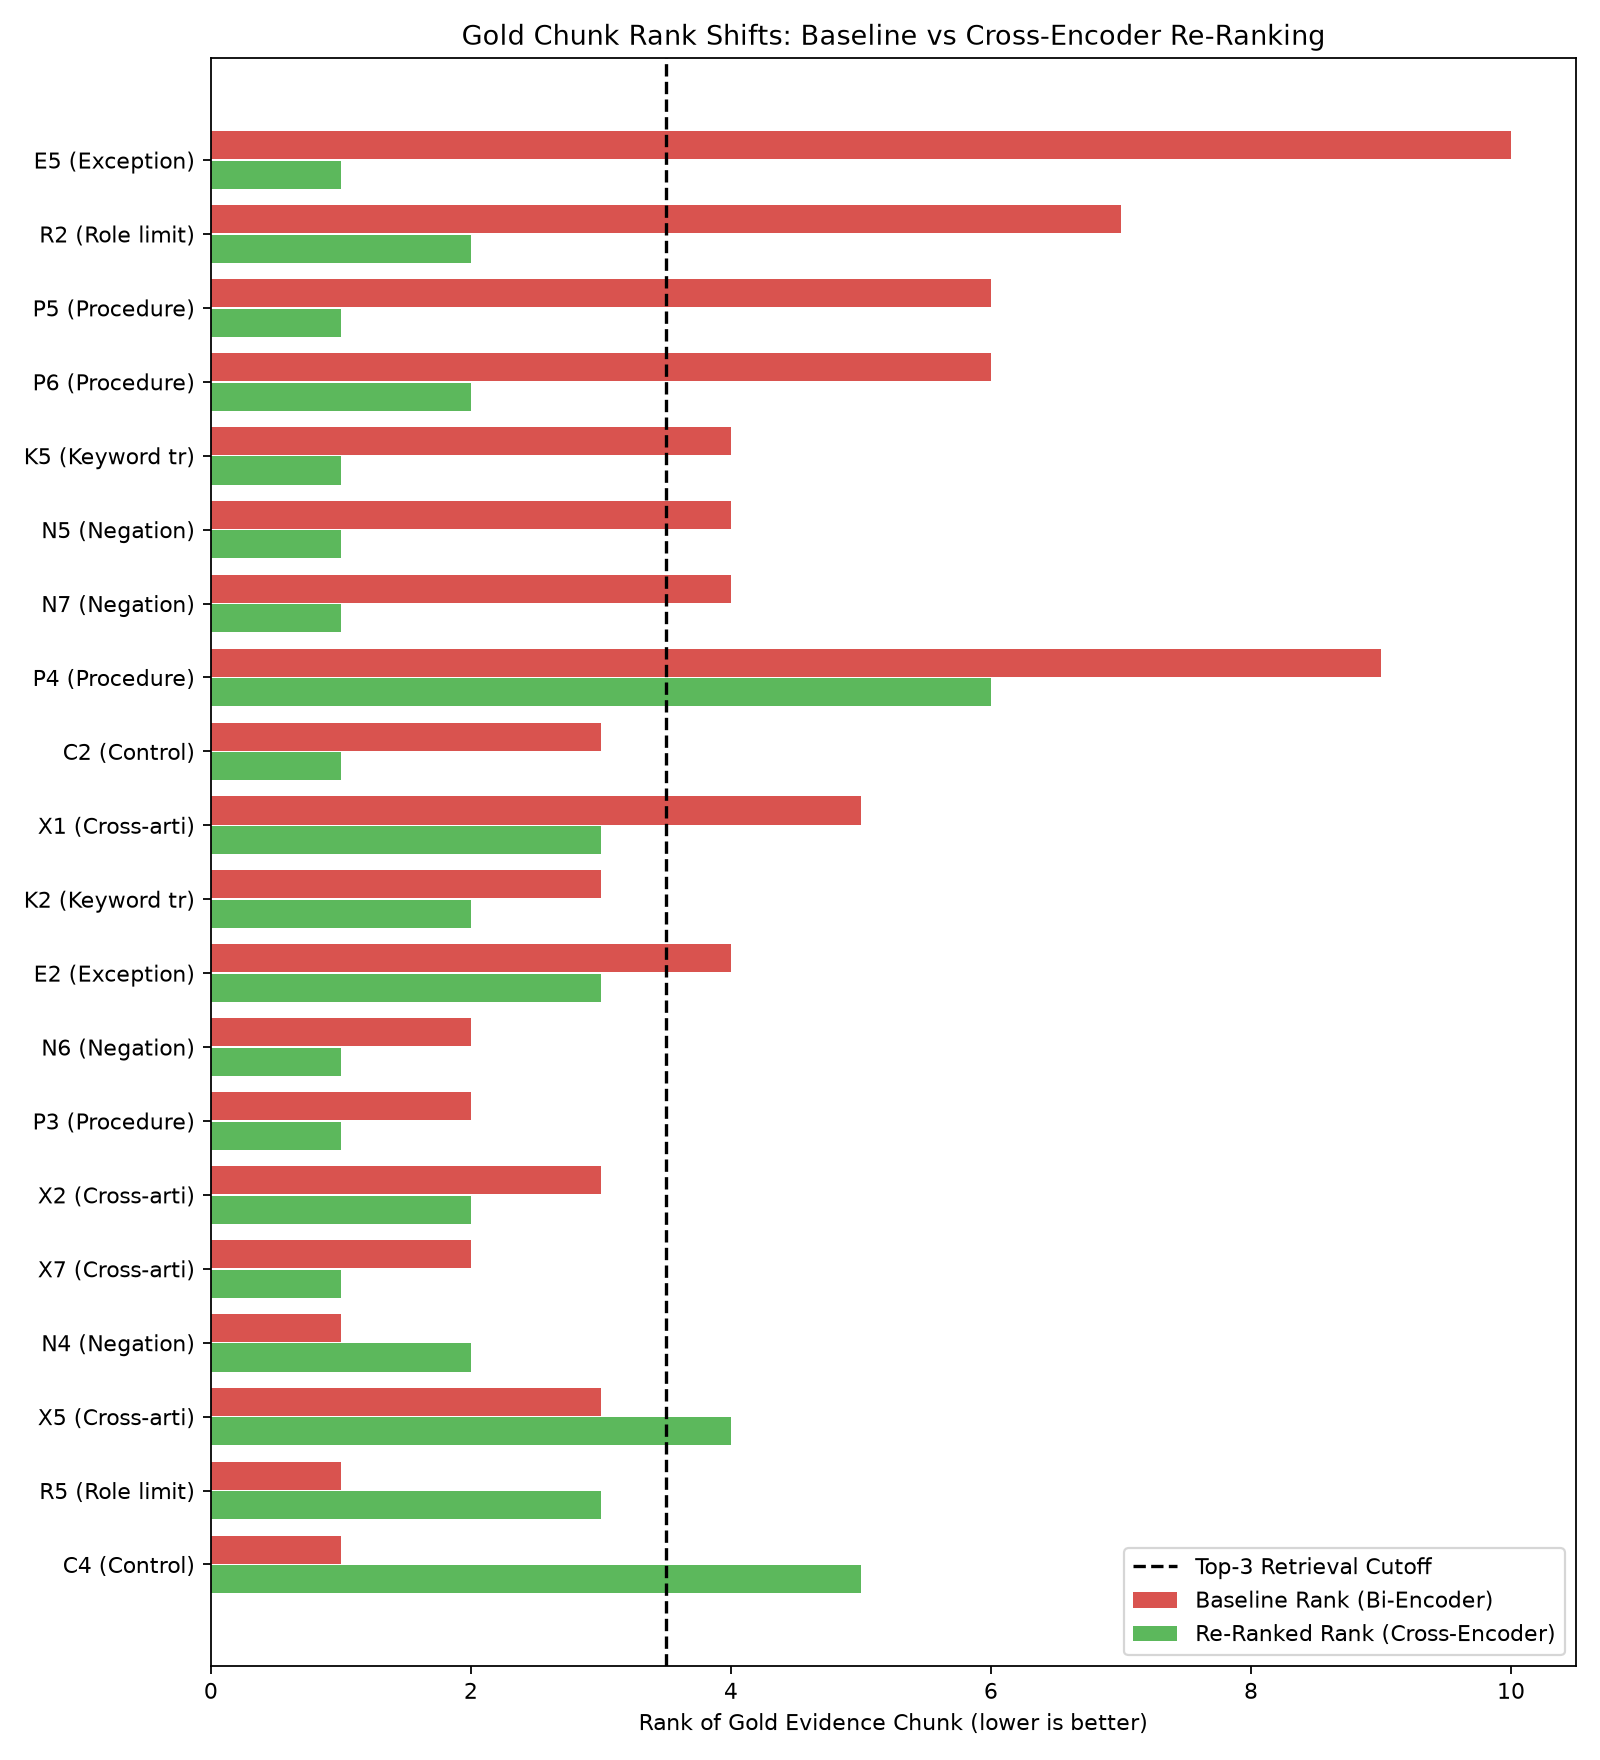
\includegraphics[width=0.48\linewidth,height=3.8cm,keepaspectratio]{results/figures/rank_shift.png}\\[-0.2em]
\captionof{figure}{Candidate rank shifts: Baseline rank vs.\ CE re-ranked rank. Green markers indicate queries successfully promoted into Top-3 (\texttt{FIXED\_BY\_RERANK}).}
\label{fig:rank_shift}
\end{tightcenter}

\textbf{Rank Shift Dynamics:} As visualized in Figure~\ref{fig:rank_shift}, CE effectively rescues queries where gold evidence was retrieved by BE but ranked outside the LLM context window (ranks 4--10). Across the 48 answerable queries, 9 queries were successfully rescued into Top-3, while only 2 experienced slight rank degradation.

\clearpage

% =================================================================================================
% PAGE 4: CASE STUDIES 1, 2, 3
% =================================================================================================
\subsection{Case Study 1: Keyword Trap / Distractor (Query K5)}
\casebox{Query K5 (Keyword Trap)}{Can police force of one State investigate in another State without permission?}{Under Seventh Schedule (Union List, Entry 80), powers of a State police force cannot be extended to another State without consent of that State Government.}{\texttt{FIXED\_BY\_RERANK} $\mid$ Rank \#4 $\rightarrow$ \#1}

\begin{tightcenter}
\scriptsize
\setlength{\tabcolsep}{3pt}
\renewcommand{\arraystretch}{0.90}
\begin{tabularx}{\textwidth}{cccrrcccX}
\toprule
\textbf{Base} & \textbf{CE} & \textbf{Shift} & \textbf{Base Sc.} & \textbf{CE Sc.} & \textbf{Gold?} & \textbf{Article} & \textbf{Page} & \textbf{Text Preview} \\
\midrule
1 & 2 & $-1$ & $0.4455$ & $-1.3391$ & no & Art. 262 & 182 & \dots water dispute of inter-state rivers \dots \\
2 & 4 & $-2$ & $0.4445$ & $-4.9825$ & no & Art. 259 & 181 & \dots Armed Forces in Part B States \dots \\
3 & 3 & $0$ & $0.4394$ & $-4.1862$ & no & Art. 131 & 92 & \dots original jurisdiction of Supreme Court \dots \\
\textbf{4} & \textbf{1} & $\mathbf{+3}$ & $0.4170$ & $\mathbf{+4.3196}$ & \textbf{YES} & \textbf{7th Sched.} & \textbf{346} & \textbf{\dots not so as to enable police to exercise jurisdiction without consent \dots} \\
5 & 7 & $-2$ & $0.4087$ & $-6.9768$ & no & 7th Sched. & 348 & \dots List II Entry 97: Residuary powers \dots \\
\bottomrule
\end{tabularx}
\vspace{0.08em}
\captionof{table}{Rank shift table for Query K5.}
\label{tab:case_k5}
\end{tightcenter}
\textbf{LLM Answer 1 (Baseline Top-3 Context):} \textit{``The provided context does not contain the answer.''} [\textbf{Score: 0.0}]. BE retrieved river disputes (Art. 262) and court jurisdiction (Art. 131) due to superficial lexical overlap with ``State'' and ``jurisdiction''.\\
\textbf{LLM Answer 2 (Re-Ranked Context):} \textit{``According to Entry 80 of the Union List in the Seventh Schedule, extension of powers of a police force to an area outside that State does not enable them to exercise jurisdiction without the consent of that State Government.''} [\textbf{Score: 1.0}]. Cross-attention promoted the true clause from Rank \#4 to Rank \#1.

\subsection{Case Study 2: Exceptions and Corner Cases (Query E5)}
\casebox{Query E5 (Exception Clause)}{Under what circumstances can Parliament legislate on a State List subject in national interest?}{Under Article 249(1), if Council of States declares by resolution supported by $\ge 2/3$ members present and voting that it is necessary in national interest.}{\texttt{FIXED\_BY\_RERANK} $\mid$ Rank \#10 $\rightarrow$ \#1}

\begin{tightcenter}
\scriptsize
\setlength{\tabcolsep}{3pt}
\renewcommand{\arraystretch}{0.90}
\begin{tabularx}{\textwidth}{cccrrcccX}
\toprule
\textbf{Base} & \textbf{CE} & \textbf{Shift} & \textbf{Base Sc.} & \textbf{CE Sc.} & \textbf{Gold?} & \textbf{Article} & \textbf{Page} & \textbf{Text Preview} \\
\midrule
1 & 4 & $-3$ & $0.6875$ & $+1.3679$ & no & Art. 246 & 176 & \dots exclusive power to make laws for List I \dots \\
2 & 2 & $0$ & $0.6588$ & $+2.1244$ & no & Art. 246 & 176 & \dots State Legislature power for State List \dots \\
3 & 3 & $0$ & $0.6384$ & $+1.7630$ & no & Art. 239AA & 145 & \dots Special provisions for NCT of Delhi \dots \\
\dots & \dots & \dots & \dots & \dots & \dots & \dots & \dots & \dots \\
\textbf{10} & \textbf{1} & $\mathbf{+9}$ & $0.5794$ & $\mathbf{+5.9311}$ & \textbf{YES} & \textbf{Art. 249} & \textbf{177} & \textbf{\dots if Council of States declared by resolution supported by $\ge 2/3$ present \dots} \\
\bottomrule
\end{tabularx}
\vspace{0.08em}
\captionof{table}{Rank shift table for Query E5.}
\label{tab:case_e5}
\end{tightcenter}
\textbf{LLM Answer 1 (Baseline Context):} Provided general distribution rule under Art. 246 rather than the national-interest exception, producing a legally incorrect answer [\textbf{Score: 0.20}].\\
\textbf{LLM Answer 2 (Re-Ranked Context):} \textit{``According to Article 249(1), Parliament can legislate on a State List subject if the Council of States passes a resolution supported by not less than two-thirds of members present and voting.''} [\textbf{Score: 1.00}]. Gold chunk surged \textbf{+9 positions (Rank \#10 $\rightarrow$ \#1)}.

\subsection{Case Study 3: Negation and Disqualification Grounds (Query N5)}
\casebox{Query N5 (Negation Clause)}{What are the specific constitutional grounds for disqualification from being an MP?}{Article 102(1) specifies 5 grounds: office of profit, unsound mind, undischarged insolvent, foreign allegiance, disqualified by law.}{\texttt{FIXED\_BY\_RERANK} $\mid$ Rank \#4 $\rightarrow$ \#1}
\textbf{LLM Answer 1 (Baseline Context):} Retrieved Art. 84 (qualifications) and Art. 191 (MLA disqualifications), confusing MPs with State legislators [\textbf{Score: 0.80}].\\
\textbf{LLM Answer 2 (Re-Ranked Context):} With Art. 102(1) promoted to \#1, LLM enumerated all five grounds (a)--(e) with complete accuracy [\textbf{Score: 1.00}].

\clearpage

% =================================================================================================
% PAGE 5: CASE STUDY 4, REGRESSIONS & ABSTENTION, LATENCY PROFILING, EMPIRICAL SCALING
% =================================================================================================
\subsection{Case Study 4: Role Limits and Numeric Thresholds (Query R2)}
\casebox{Query R2 (Role Limit)}{What is the minimum age to become a member of the Council of States?}{Article 84(b) fixes minimum age at 30 years for Rajya Sabha (vs 25 years for House of the People).}{\texttt{FIXED\_BY\_RERANK} $\mid$ Rank \#7 $\rightarrow$ \#2}
\textbf{LLM Answer 1 (Baseline Context):} Retrieved composition (Art. 80) and duration (Art. 83). The age threshold sat at Rank \#7, forcing LLM abstention [\textbf{Score: 0.00}].\\
\textbf{LLM Answer 2 (Re-Ranked Context):} CE elevated Art. 84 to Rank \#2, enabling direct answer: \textit{``According to Article 84, not less than thirty years of age.''} [\textbf{Score: 1.00}].

\subsection{Documented Regressions \& Abstention Performance}
\begin{itemize}
  \setlength{\itemsep}{0.5pt}\setlength{\parskip}{0pt}
  \item \textbf{Regressions (C4, X5):} In Query C4 (Lok Sabha duration), gold chunk demoted from \#1 to \#5 because CE favored emergency extension clauses over standard term provisions. In X5 (Retirement age SC vs.\ HC), gold chunk dropped from \#3 to \#4 due to competing High Court articles.
  \item \textbf{Abstention Validation (U1--U7):} All 7 unanswerable queries achieved \textbf{100\% abstention accuracy} (\textit{``The provided context does not contain the answer.''}), confirming that strict negative constraints in system prompt eliminate hallucination when evidence is absent.
\end{itemize}

\section{Latency Profiling and End-to-End Runtime}
\label{sec:latency}
Table~\ref{tab:latency_profile} details stage-wise latencies measured across 5 repeats per query following warm-up.

\begin{tightcenter}
\small
\setlength{\tabcolsep}{5pt}
\renewcommand{\arraystretch}{0.92}
\begin{tabular}{lrr}
\toprule
\textbf{Pipeline Stage} & \textbf{Median Latency} & \textbf{Mean Latency} \\
\midrule
Query Embedding (\texttt{all-MiniLM-L6-v2}) & $9.88$\,ms & $9.72$\,ms \\
FAISS Index Search (\texttt{IndexFlatIP}, $N = 880$) & $0.14$\,ms & $0.14$\,ms \\
\textbf{Total Baseline Retrieval Latency} & $\mathbf{10.02}$\,\textbf{ms} & $\mathbf{9.85}$\,\textbf{ms} \\
\midrule
CE Scoring ($k = 10$ candidate pairs) & $324.97$\,ms & $322.03$\,ms \\
\textbf{Total Re-Rank Retrieval Latency} & $\mathbf{333.98}$\,\textbf{ms} & $\mathbf{331.88}$\,\textbf{ms} \\
\midrule
LLM Generation Answer 1 (Top-3, Llama-3.2) & $13,160.00$\,ms & $14,654.86$\,ms \\
LLM Generation Answer 2 (Re-ranked, Llama-3.2) & $12,740.00$\,ms & $13,454.29$\,ms \\
\midrule
\textbf{End-to-End Baseline (Retrieval + LLM)} & $\mathbf{13.17}$\,\textbf{sec} & $\mathbf{14.66}$\,\textbf{sec} \\
\textbf{End-to-End Re-Ranked (Retrieval + LLM)} & $\mathbf{13.07}$\,\textbf{sec} & $\mathbf{13.78}$\,\textbf{sec} \\
\bottomrule
\end{tabular}
\vspace{0.10em}
\captionof{table}{Stage-wise runtime profiling per query.}
\label{tab:latency_profile}
\end{tightcenter}

\textbf{Runtime Analysis:} First-stage BE vector search executes in $10.02$\,ms ($9.88$\,ms query encoding + $0.14$\,ms FAISS inner product scan over 880 chunks). Second-stage CE scoring adds $324.97$\,ms across $k=10$ candidate pairs ($32.5$\,ms per pair). Crucially, autoregressive token generation by local LLM dominates overall turnaround time ($\approx 13$\,s, accounting for $97.5\%$ of execution time). Thus, CE re-ranking overhead represents $< 2.5\%$ of user-perceived latency while delivering $+14.6\%$ improvement in Hit@3.

\section{Scaling Question: Why Not Cross-Encode Everything?}
\label{sec:scaling}
The assignment asks: \textit{Why do we not simply run a CE across the entire document collection from the start?}

\subsection{Empirical Benchmark \& Extrapolation}
Table~\ref{tab:empirical_scaling} presents empirical CPU measurements across increasing subsets of the Constitution ($N=10$ to $N=880$), and Table~\ref{tab:extrapolation} projects latencies to enterprise collection sizes based on measured inference constants ($34.5$\,ms/pair for CE; $0.057$\,$\mu$s/vector for FAISS inner products).

\begin{tightcenter}
\footnotesize
\setlength{\tabcolsep}{4.5pt}
\renewcommand{\arraystretch}{0.92}
\begin{tabular}{rrrrr}
\toprule
\textbf{Corpus Size ($N$)} & \textbf{FAISS Median} & \textbf{FAISS Std} & \textbf{CE Median} & \textbf{CE Std} \\
\midrule
$10$ & $0.007$\,ms & $0.005$\,ms & $346.26$\,ms & $5.88$\,ms \\
$50$ & $0.009$\,ms & $0.006$\,ms & $1,647.41$\,ms & $12.96$\,ms \\
$100$ & $0.011$\,ms & $0.007$\,ms & $3,455.23$\,ms & $23.76$\,ms \\
$250$ & $0.018$\,ms & $0.009$\,ms & $7,924.89$\,ms & $23.82$\,ms \\
$500$ & $0.023$\,ms & $0.012$\,ms & $15,840.80$\,ms & $80.78$\,ms \\
$\mathbf{880}$ \textbf{(Full)} & $\mathbf{0.050}$\,\textbf{ms} & $0.016$\,ms & $\mathbf{30,359.15}$\,\textbf{ms} & $61.24$\,ms \\
\bottomrule
\end{tabular}
\vspace{0.08em}
\captionof{table}{Empirical scaling latency: FAISS IndexFlatIP vs.\ CE across corpus sizes.}
\label{tab:empirical_scaling}
\end{tightcenter}

\clearpage

% =================================================================================================
% PAGE 6: SCALING PLOT, THEORETICAL EXTRAPOLATION, INTRACTABILITY, CONCLUSION
% =================================================================================================
\begin{tightcenter}
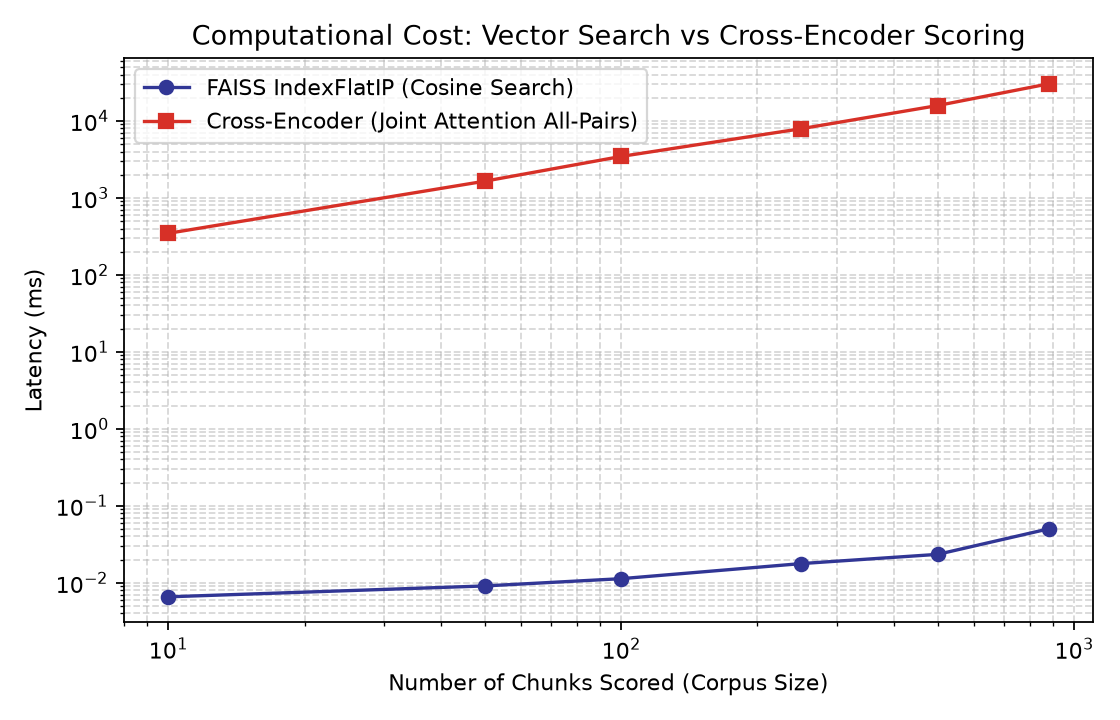
\includegraphics[width=0.48\linewidth,height=3.8cm,keepaspectratio]{results/figures/scaling.png}\\[-0.2em]
\captionof{figure}{Scaling latency comparison: FAISS Flat vector search vs.\ Exhaustive CE. Full-corpus CE exhibits steep linear growth that quickly becomes computationally prohibitive.}
\label{fig:scaling}
\end{tightcenter}

\begin{tightcenter}
\footnotesize
\setlength{\tabcolsep}{5pt}
\renewcommand{\arraystretch}{0.92}
\begin{tabular}{rccc}
\toprule
\textbf{Corpus Chunks} & \textbf{FAISS Flat Search} & \textbf{Exhaustive CE} & \textbf{Two-Stage ($k=10$)} \\
\midrule
$10,000$ & $0.57$\,ms & $344.99$\,s ($5.7$\,minutes) & $334$\,ms \\
$100,000$ & $5.70$\,ms & $3,449.90$\,s ($57.5$\,minutes) & $338$\,ms \\
$1,000,000$ & $56.99$\,ms & $34,499.04$\,s (\textbf{9.6 hours}) & $389$\,ms \\
$10,000,000$ & $569.95$\,ms & $344,990.39$\,s (\textbf{4.0 days}) & $895$\,ms \\
\bottomrule
\end{tabular}
\vspace{0.08em}
\captionof{table}{Theoretical scaling extrapolation: Exhaustive CE vs.\ Two-Stage RAG.}
\label{tab:extrapolation}
\end{tightcenter}

\subsection{Why Exhaustive CE is Intractable}
\begin{enumerate}
  \setlength{\itemsep}{0.5pt}\setlength{\parskip}{0pt}
  \item \textbf{Inability to Precompute Document Representations:} BEs decouple query and document representations into $\mathbf{u}_q = f_\theta(q)$ and $\mathbf{v}_d = g_\theta(d)$. This allows all $N$ document encodings to be computed offline once and indexed. In contrast, CE requires joint input pairs $(q, d)$ passed through all transformer layers simultaneously. Thus, \textbf{every incoming query requires $N$ online transformer forward passes}, destroying interactive query throughput.
  \item \textbf{Quadratic Attention Overhead:} For query length $L_q = 20$ tokens and document chunk length $L_d = 200$ tokens, self-attention complexity scales quadratically with total sequence length: $\mathcal{O}((L_q + L_d)^2) = (220)^2 = 48,400$ token-pair attention weights per chunk across all 6 transformer layers. In contrast, a BE evaluates a 384-dimensional dot product requiring only 384 multiply-accumulate operations ($0.057$\,$\mu$s).
  \item \textbf{Incompatibility with Spatial Vector Indexing:} Vector search algorithms (such as FAISS IVF, HNSW, or ScaNN) exploit spatial triangle inequalities and clustering to prune vector space exploration from $\mathcal{O}(N)$ down to $\mathcal{O}(\log N)$. CE scalar scores are query-dependent non-metric outputs that cannot be indexed into spatial trees or geometric graphs, mandating brute-force $\mathcal{O}(N)$ comparisons.
\end{enumerate}

\subsection{Architectural Synthesis and Deployment Recommendations}
In real-world legal and enterprise RAG deployments, scaling constraints dictate a clear architectural design:
\begin{itemize}
  \setlength{\itemsep}{0.5pt}\setlength{\parskip}{0pt}
  \item \textbf{First-Stage Candidate Pruning ($N \rightarrow k$):} Utilize ANN indexing (e.g., FAISS HNSW or ScaNN) to retrieve a bounded candidate set ($k \in [10, 20]$). Dot products on normalized vectors preserve sub-millisecond query latencies even at million-scale document corpora.
  \item \textbf{Second-Stage Re-Ranking ($k \rightarrow 3$):} Limit CE inference strictly to the retrieved candidate pool. This bounds transformer forward passes to a constant $k \times \mathcal{O}(L^2)$, eliminating corpus-size dependency from the re-ranking latency budget.
  \item \textbf{Strict Negative Prompting:} Constrain downstream LLM with affirmative citation rules and explicit abstention triggers to completely suppress hallucinations when relevant context is absent.
\end{itemize}

\textbf{Conclusion:} Decoupled two-stage retrieval---pruning $N \rightarrow 10$ candidates via a BE in sub-millisecond time ($0.14$\,ms), and scoring those 10 candidates with a CE ($325$\,ms)---is the required architectural compromise between accuracy and latency. It captures $90\%$ of available candidates into top-3 hits, rescues $18.8\%$ of buried queries, and achieves $+14.6\%$ Hit@3 with negligible turnaround impact.

\end{document}
